\documentclass{beamer}

\usepackage{listings}
\usepackage{xcolor}
\usepackage{multicol}
\usepackage{amsmath}

\definecolor{codegreen}{rgb}{0,0.6,0}
\definecolor{codegray}{rgb}{0.5,0.5,0.5}
\definecolor{codepurple}{rgb}{0.58,0,0.82}
\definecolor{backcolour}{rgb}{0.95,0.95,0.92}

\lstdefinestyle{mystyle}{
    %backgroundcolor=\color{backcolour}, 
    commentstyle=\color{codegreen},
    keywordstyle=\color{magenta},
    numberstyle=\tiny\color{codegray},
    stringstyle=\color{codepurple},
    basicstyle=\ttfamily\footnotesize,
    breakatwhitespace=false,         
    breaklines=true,                 
    captionpos=b,                    
    keepspaces=true,                 
    numbers=left,                    
    numbersep=5pt,                  
    showspaces=false,                
    showstringspaces=false,
    showtabs=false,                  
    tabsize=2
}

\lstset{style=mystyle}

\usepackage{hyperref}
\hypersetup{
    colorlinks=true,
    linkcolor=blue,
    filecolor=magenta,      
    urlcolor=cyan
}

\urlstyle{same}

%Information to be included in the title page:
\title{1: Introduction to Competitive Programming}
\author{CPCFI}
\institute{UNAM's School of Engineering}
\date{2021 \\ \vspace{0.5cm} \scriptsize{Based on: Halim S., Halim F.\textit{Competitive Programming 3}}. Handbook for ACM ICPC and IOI Contestants. 2013}

\begin{document}
\frame{\titlepage}
\AtBeginSection[]
{
  \begin{frame}
    \frametitle{Table of Contents}
    \tableofcontents[currentsection]
  \end{frame}
}

%----------------------------------------------------------------------
%----------------------------------------------------------------------
%----------------------------------------------------------------------
\section{1. Competitive Programming}
\begin{frame}{Competitive Programming}
    \begin{itemize}
        \item \textbf{CP?}:
            \begin{quote}
                Given a well-known Computer Science problem, solve it as quickly as possible!
            \end{quote}
        \item \textbf{Objective}:
            \begin{quote}
                The true end goal is to produce all-rounder computer scientists/programmers who are much readier to produce better software and to face harder CS research problems in the future
            \end{quote}
    \end{itemize}
\end{frame}

\begin{frame}{CP Problems}
    \begin{figure}
        \centering
        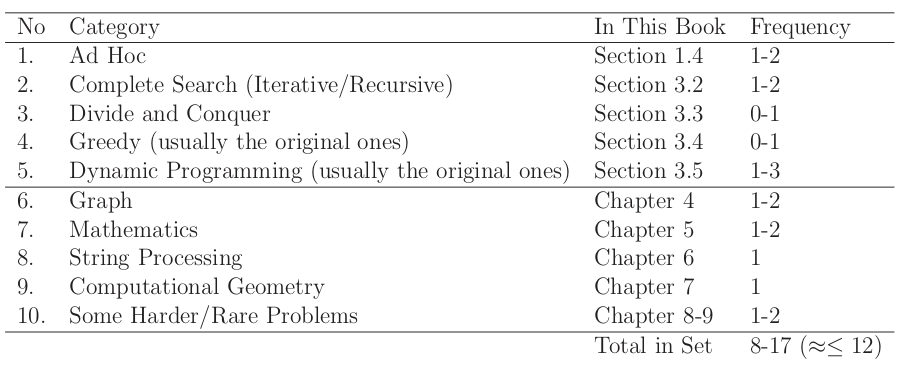
\includegraphics[scale=0.3]{imgs/1-CompetitiveProgramming/cp_problems.png}
        \caption{ACM ICPC (Asia) Problem Types. See \cite{Halim}}
        \label{fig:CP_problems_categories}
    \end{figure}
\end{frame}

\begin{frame}{CP Programmer POV}
    \begin{figure}
        \centering
        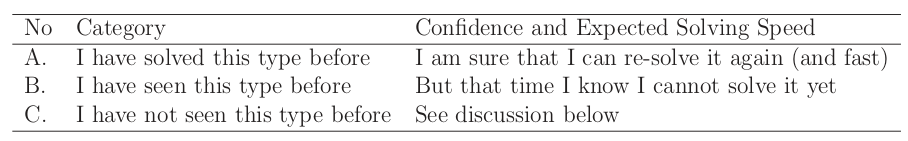
\includegraphics[scale=0.3]{imgs/1-CompetitiveProgramming/cp_expected_abilities.png}
        \caption{Problem Types. See \cite{Halim}}
        \label{fig:CP_problem_categories_programmer_POV}
    \end{figure}
\end{frame}

\begin{frame}{Algorithm Analysis}
    \begin{quote}
        Given the maximum input bound, can the currently developed algorithm, with its time/space complexity, pass the time/memory limit given for that particular problem?
    \end{quote}
\end{frame}

\begin{frame}{Algorithm Analysis}
    Computers can run $10^8$ operations per second \footnote{$10^8 = 100,000,000 = 100M$}. We can use this information to know if our algorithm will run in time. 
    
    Examples:
    \begin{itemize}
        \item Input size: $n=10^5$. Algorithm complexity: $O(n^2)$. Time: $O(n^2) = (10^5)^2 = 10^{10}$. The algorithm will need hundreds of seconds to finish
        \item If the algorithm complexity is: $O(n\log_2n)$, then time would be: $10^5\log_210^5 \approx 1.7\times 10^6$ which will pass the time limit
    \end{itemize}
    
    The algorithm complexity will decide if its worth it to implement a certain algorithm or not. 
    \begin{quote}
        Start coding an algorithm only when you know it is correct and fast enough
    \end{quote}
\end{frame}

\begin{frame}{Time Complexities for $n$ input}
    \begin{figure}
        \centering
        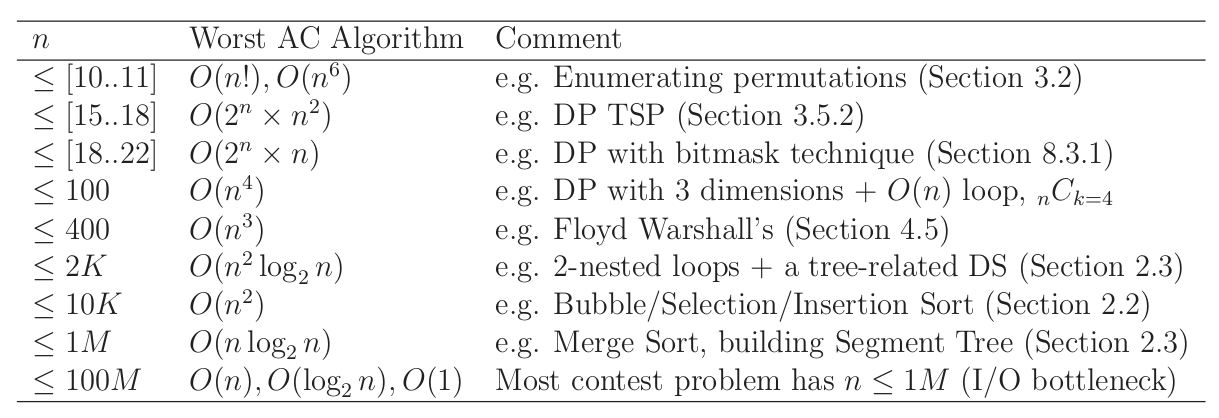
\includegraphics[scale=0.25]{imgs/1-CompetitiveProgramming/rule_of_thumb_complexities.png}
        \caption{Time complexities for a given $n$}
        \label{fig:my_label_20}
    \end{figure}
\end{frame}

\begin{frame}{Code Testing}
    Guidelines for designing good test cases:
    \begin{enumerate}
        \item Your test cases should include the sample test cases since the sample output is guaranteed to be correct
        \item For problems with multiple test cases in a single run, you should include two identical sample test cases consecutively in the same run. This helps to determine if you have forgotten to initialize any variables
        \item Your test cases should include tricky corner cases. Corner cases typically occur at extreme values such as N = 0, N = 1, negative values, large final (and/or intermediate) values that does not fit 32-bit signed integer, etc.
    \end{enumerate}
\end{frame}

\begin{frame}{Code Testing}
    \begin{enumerate}
      \setcounter{enumi}{3}
        \item Your test cases should include large cases. Increase the input size incrementally up to the maximum input bounds stated in the problem description. Sometimes your program may work for small test cases, but produces wrong answer, crashes, or exceeds the time limit when the input size increases.
        \item Do not assume that the input will always be nicely formatted if the problem description does not explicitly state it. Try inserting additional whitespace (spaces, tabs) in the input and test if your code is still able to obtain the values correctly without crashing.
    \end{enumerate}
\end{frame}

\begin{frame}{Practice}
    \begin{figure}
        \centering
        
\includegraphics[scale=0.3]{imgs/1-CompetitiveProgramming/uva_logo.png}
        \caption{\url{https://onlinejudge.org/index.php?option=com_onlinejudge&Itemid=8&category=604}}
        \label{fig:my_label_11}
    \end{figure}
    
    \begin{figure}
        \centering
        
\includegraphics[scale=0.5]{imgs/1-CompetitiveProgramming/icpc_logo.png}
        \caption{\url{https://icpc.global/compete/problems}}
        \label{fig:my_label_10}
    \end{figure}
\end{frame}

\begin{frame}{Getting Started: Anatomy of a problem}
    \begin{itemize}
        \item Background story/problem description
        \item Input and Output description
        \item Sample Input and Sample Output
        \item Hints or Footnotes
    \end{itemize}
\end{frame}

%----------------------------------------------------------------------
%----------------------------------------------------------------------
%----------------------------------------------------------------------
\section{1.2 C++}

\begin{frame}{C++}
    The C++ Programming Language fourth edition. Bjarne Stroustrup
    \begin{itemize}
        \item Part I: Chapters 2-5
        \item Part IV: The Standard Library (STL)
    \end{itemize}
\end{frame}

\begin{frame}[fragile]{I/O}
Problem: output the sum of numbers on each case
\begin{itemize}
    \item Case 1: $n$ input cases
\begin{lstlisting}
Sample Input | Sample Output
----------------------------
3            | 3
1 2          | 12
5 7          | 9
6 3          |
----------------------------
\end{lstlisting}
    \item Case 2: Stop until $0$ $0$
\begin{lstlisting}
Sample Input | Sample Output
----------------------------
1 2          | 3
5 7          | 12
6 3          | 9
0 0          |
----------------------------
\end{lstlisting}
\end{itemize}
\end{frame}

\begin{frame}[fragile]{I/O}
    \begin{itemize}
        \item Case 3: Stop until \verb|EOF|
\begin{lstlisting}
Sample Input | Sample Output
----------------------------
1 2          | 3
5 7          | 12
6 3          | 9
----------------------------
\end{lstlisting}
        \item Case 4: Each case indicates the number of elements to sum
\begin{lstlisting}
Sample Input | Sample Output
----------------------------
1 1          | 1
2 3 4        | 7
3 8 1 1      | 10
4 7 2 9 3    | 21
5 1 1 1 1 1  | 5
----------------------------
\end{lstlisting}
    \end{itemize}
\end{frame}

\begin{frame}[fragile]{I/O C++ code}
    \begin{itemize}
        \item Case 1
\begin{lstlisting}[language=c++]
#include <stdio.h>
int main() {
	int TC, a, b;
	scanf("%d", &TC);
	while (TC--) {
		scanf("%d %d", &a, &b);
		printf("%d\n", a + b);
	}
}
\end{lstlisting}
        \item Case 2
\begin{lstlisting}[language=c++]
#include <stdio.h>
int main() {
	int a, b;
	while (scanf("%d %d", &a, &b), (a || b)) {
		printf("%d\n", a + b);
	}
}
\end{lstlisting}
    \end{itemize}
\end{frame}

\begin{frame}[fragile]{I/O C++ code}
    \begin{itemize}
        \item Case 3
\begin{lstlisting}[language=c++]
#include <stdio.h>
int main() {
	int a, b;
	while (scanf("%d %d", &a, &b) != EOF) {
		printf("%d\n", a + b);
	}
}
\end{lstlisting}
        \item Case 4
\begin{lstlisting}[language=c++]
#include <stdio.h>
int main() {
	int k;
	while (scanf("%d", &k) != EOF) {
		int v, ans = 0;
		while (k--) {
			scanf("%d", &v);
			ans += v;
		}
		printf("%d\n", ans);
	}
}
\end{lstlisting}
    \end{itemize}
\end{frame}

%----------------------------------------------------------------------
%----------------------------------------------------------------------
%----------------------------------------------------------------------
\section{1.3 Time to Start the Journey}

\begin{frame}{Time to Start the Journey}
    \begin{quote}
        What we have to learn to do, we learn by doing. 
        \vspace{0.3cm} \\
        
          - Aristotle, Nichomachean Ethics
    \end{quote}
\end{frame}

\begin{frame}{UVa - Competitive Programming 3}
    
    University of Valladolid's Online Judge: 
    
    \url{https://onlinejudge.org/index.php?option=com_onlinejudge&Itemid=8&category=604}
    
    \begin{itemize}
        \item Most of these problems only need a basic computer science knowledge to code a solution
        \item UVa: \textbf{CP3 $>$ Introduction $>$ Getting Started: The Easy Problems}
    \end{itemize}
\end{frame}


%----------------------------------------------------------------------
%----------------------------------------------------------------------
%----------------------------------------------------------------------
\section{1.4 Ad Hoc Problems}

\begin{frame}{Ad Hoc Problems}
    \begin{quote}
        Ad Hoc problems are problems that ‘cannot be classified anywhere else’ since each problem description and its corresponding solution are ‘unique’.
    \end{quote}
    \begin{itemize}
        \item Ad Hoc problems frequently appear in programming contests. In ICPC, $\approx 1-2$ problems out of every $\approx 10$ problems are Ad Hoc problems
        \item If the Ad Hoc problem is easy, it will usually be the first problem solved by the teams in a programming contest
        \item In an ICPC regional contest with about 60 teams, your team would rank in the lower half (rank 30-60) if you can only solve Ad Hoc problems
        \item Most Ad Hoc problems can be solved without using advanced data structures or algorithms
    \end{itemize}
\end{frame}

\begin{frame}{Ad Hoc Categories}
    \begin{itemize}
        \item Cards
        \item Chess
        \item Other games
        \item Palindromes
        \item Anagrams
        \item Interesting real life problems
        \item Dates and time
        \item Time Wasters
    \end{itemize}
\end{frame}

\begin{frame}{UVa - Competitive Programming 3}
    
    University of Valladolid's Online Judge: 
    
    \url{https://onlinejudge.org/index.php?option=com_onlinejudge&Itemid=8&category=604}
    
    \begin{itemize}
        \item Most of these problems only need a basic computer science knowledge to code a solution
        \item UVa: \textbf{CP3 $>$ Introduction $>$ Ad Hoc Problems}
    \end{itemize}
\end{frame}


%----------------------------------------------------------------------
%----------------------------------------------------------------------
%----------------------------------------------------------------------
\section{2.2 Linear Data Structures}

\begin{frame}{Importance of Data Structures}
    \begin{itemize}
        \item Most problems can be solved in many ways, however, using an efficient or the most proper data structure can be the difference between an accepted solution or a time limit exceeded solution
        \item The knowledge required must be such that given a problem, one should identify the correct DS to use
        \item Aim to understand the following concepts from each DS:
            \begin{itemize}
                \item Strengths/Weaknesses
                \item Time/Space complexities
            \end{itemize}
    \end{itemize}
\end{frame}

\begin{frame}{Linear Data Structures}
    \begin{itemize}
        \item \underline{\textbf{Def:}} a data structure in which its elements form a linear sequence (from left to right or top to bottom)
        
        \item LDS: 
        \begin{itemize}
            \item \color{blue} Static Array \color{black}
            \item \color{blue} Dynamically-Resizeable Array \color{black}
            \item \color{blue} Linked List \color{black}
			\item \color{blue} Doubly Linked List \color{black}
            \item \color{blue} Stack \color{black}
            \item \color{blue} Queue \color{black}
            \item \color{blue} Doubly Linked List \color{black}
            \item Double-ended Queue (Deque)
            \item Bitset
            \item Bitmasks (lighweight small sets of Booleans)
        \end{itemize}
        \item \url{https://visualgo.net/en}
    \end{itemize}
\end{frame}

\begin{frame}[fragile]
\frametitle{But first...common background for most LDS}
	List Abstract Data Type (ADT) is a sequence of items where positional order is important: $$a_0, a_1, \ldots, a_{n-2}, a_{n-1}$$
	Common operations among lists:
	\begin{enumerate}
		\item \verb|get(i)|: returns $a_i$ ($0$-based indexed)
		\item \verb|search(v)|: decide if item $v$ exists in the list. If true, also report its index, otherwise, return \verb|-1|
		\item \verb|insert(i, v)|: inserts item $v$ at index $i$; possibly shifting elements in the range $[i,\ldots, n-1]$ to the right one position
		\item \verb|remove(i)|: removes item at index $i$ in the list; possibly shifting elements in the range $[i+1, \ldots, n-1]$ to the left one position
	\end{enumerate}
\end{frame}

%----------------------------------------------------------------------
%----------------------------ARRAY-------------------------------------
%----------------------------------------------------------------------
\begin{frame}{Static Array}
	\begin{figure}
		\centering
		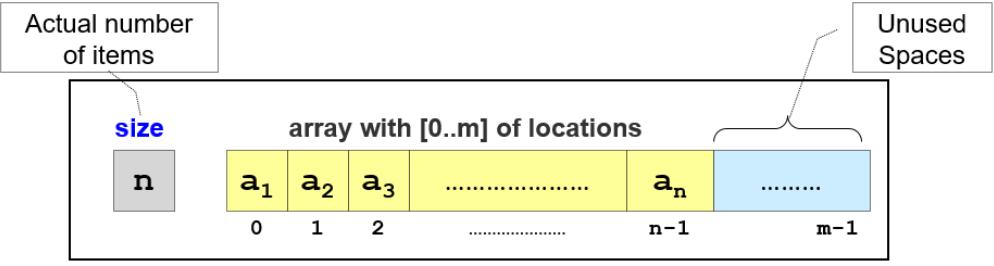
\includegraphics[scale=0.6]{imgs/2-LDS/array/array.png}
	\end{figure}
\end{frame}

\begin{frame}{Static Array}
	Great candidate for implementing a List ADT !
	\begin{figure}
		\centering
		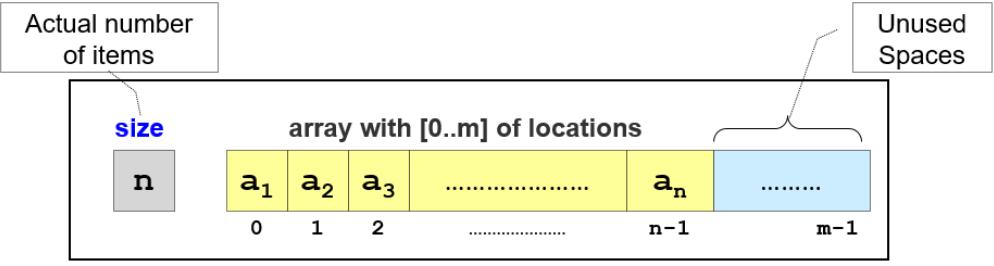
\includegraphics[scale=0.4]{imgs/2-LDS/array/array.png}
		\caption{List ADT implementation using Array}
	\end{figure}
	Compact array: 
	\begin{itemize}
		\item $[0,\ldots,n-1]$ indices are occupied
		\item $[n,\ldots,m-1]$ indices are empty
	\end{itemize}
\end{frame}

\begin{frame}[fragile]
\frametitle{Static Array: Operations}
	Let $A$ be a static array with indices \verb|[0,...,n-1]| occupied:
	\begin{itemize}
		\item \verb|get(i)|: return \verb|A[i]|
		\item \verb|search(v)|: check each index one by one to see if \verb|A[i] == v|. Return \verb|i| if \verb|true|, otherwise, return \verb|-1|
		\item \verb|insert(i, v)|: shift elements in range \verb|[i,...,n-1| one place to the right and set \verb|A[i] = v|
		\item \verb|remove(i)|: shift elements in range \verb|[i+1,...,n-1]| one place to the left
	\end{itemize}
\end{frame}

\begin{frame}[fragile]
\frametitle{Static Array: Time complexity}
		\begin{itemize}
		\item \verb|get(i)|: \color{red}$O(1)$\color{black}
		\item \verb|search(v)|: \color{red}$O(n)$\color{black}
		\item \verb|insert(i, v)|: \color{red}$O(n)$\color{black}
		\item \verb|remove(i)|: \color{red}$O(n)$\color{black}
	\end{itemize}
\end{frame}

\begin{frame}[fragile]
\frametitle{Static Array: Problems}
	\begin{itemize}
		\item Size is static and it may be a problem if the number of elements to be stored is not known in advance
		\item \verb|insert| and \verb|remove| operations are too expensive because elements are contiguously stored in memory
	\end{itemize}
\end{frame}

%----------------------------------------------------------------------
%----------------------------DYBAMIC ARRAY-----------------------------
%----------------------------------------------------------------------
\begin{frame}[fragile]{Dynamically-Resizeable Array}
    \begin{figure}
        \centering
        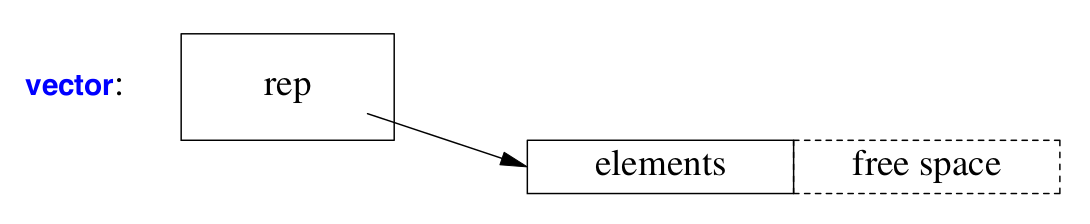
\includegraphics[scale=0.28]{imgs/2-LDS/vector.png}
    \end{figure}
\end{frame}

\begin{frame}[fragile]{Dynamically-Resizeable Array}
    \begin{itemize}
    	\item Solves the problems encountered with \verb|array|
        \item Handles runtinme resizing
        \item Better to use a \textbf{vector} if the input size is unknown.               \begin{quote}
                    Use it unless you have a good reason not to
                \end{quote}
     \end{itemize}
     
      \begin{figure}
	    \centering
        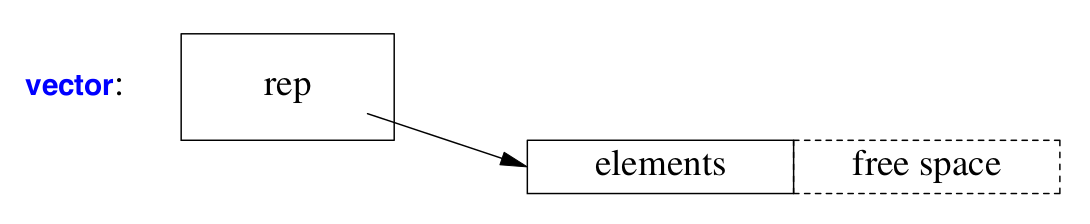
\includegraphics[scale=0.25]{imgs/2-LDS/vector.png}
        \label{fig:vector}
	  \end{figure}
	  
	  \begin{itemize}
        \item \textbf{C++}: \verb|STL::vector|
        \item \color{red}\verb|C++| code: \verb|ch2_01_array_vector.cpp|\color{black}
    \end{itemize}
\end{frame}

\begin{frame}[fragile]{Dynamically-Resizeable Array: Operations}
    \begin{itemize}
        \item \textbf{Sort} : \url{https://visualgo.net/en/sorting}
            \begin{itemize}
                \item $O(n^2)$: slow, bad idea ! 
                \item $O(n\log n)$: default choice in programming contests. Use \verb|stable_sort| or \verb|partial_sort| from C++ \verb|STL algorithm| library
                \item $O(n)$: can be used if the data has special properties
            \end{itemize}
        \item \textbf{Search}
            \begin{itemize}
                \item $O(n)$ Linear Search: avoid whenever as possible
                \item $O(\log n)$ Binary Search: data must be sorted first in order to use this algorithm. Consider using \verb|C++ STL algorithm binary_search()|, \verb|lower_bound()| or \verb|upper_bound()|
                \item $O(1)$ using Hashes
            \end{itemize}
        \item \color{red}\verb|C++| code: \verb|ch2_02_algorithm_collections.cpp|\color{black}
    \end{itemize}
\end{frame}

%----------------------------------------------------------------------
%----------------------------LINKED LIST-------------------------------
%----------------------------------------------------------------------
\begin{frame}[fragile]
\frametitle{Linked List}
	\begin{figure}
		\centering
		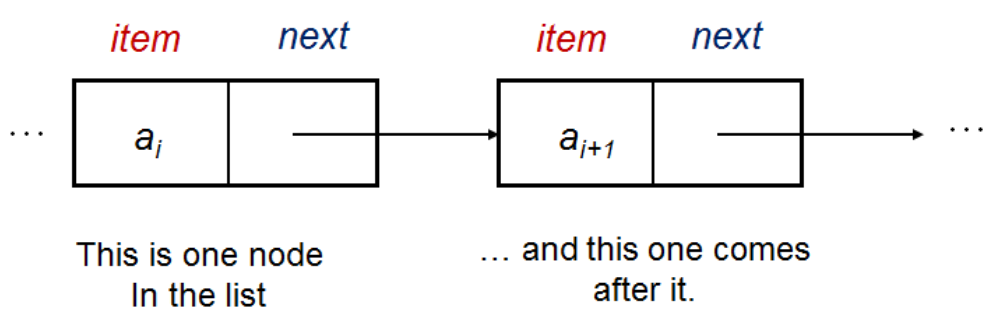
\includegraphics[scale=0.5]{imgs/2-LDS/linked-list/linked-list.png}
	\end{figure}	
\end{frame}

\begin{frame}[fragile]{Linked List}
    \begin{itemize}
        \item Uses pointers to store items non-contiguously in memory
    \end{itemize}
    \begin{figure}[H]
        \centering
        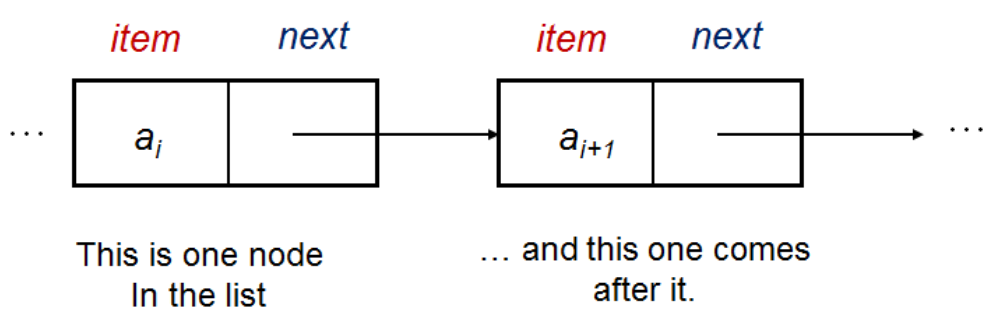
\includegraphics[scale=0.28]{imgs/2-LDS/linked-list/linked-list.png}
        \caption{Linked list}
    \end{figure}
    
	\begin{lstlisting}[language=c++]
struct Vertex {
	int item;
	Vertex* next;
};
\end{lstlisting}
	In addition to this, we need to add two more pointers: \verb|head| and \verb|tail| that should point to the first and last elements of the linked list respectively
\end{frame}

\begin{frame}[fragile]
\frametitle{Linked List: Operations}
	\begin{itemize}
		\item \verb|get(i)|: starting from \verb|head| pointer, iterate until index \verb|i|
		\item \verb|search(v)|: starting from \verb|head| pointer, iterate until finding \verb|item == v|
		\item Insertion \verb|insert(i, v)|
			\begin{itemize}
				\item At an empty LL
				\item At the head of the LL (\verb|i=0|)
				\item In between the head and the tail (\verb|i=[1,...,n-1]|)
				\item At the tail of the LL (\verb|i=n|)
			\end{itemize}
		\item Removal \verb|remove(i)|
			\begin{itemize}
				\item At the head of the LL (\verb|i=0|)
				\item In between the head and the tail (\verb|i=[1,...,n-2]|)
				\item At the tail of the LL (\verb|i=n-1|)
			\end{itemize}
	\end{itemize}
\end{frame}


\begin{frame}[fragile]
\frametitle{Linked List: Time Complexity}
	\begin{itemize}
		\item \verb|get(i)|: \color{red}$O(n)\quad$\color{black} since it should traverse through all the elements until item \verb|i|
		\item \verb|search(v)|: \color{red}$O(n)$\color{black}
		\item \verb|insert(i, v)|: \color{red}$O(n)$\color{black}
		\item \verb|remove(i)|: \color{red}$O(n)$\color{black}
	\end{itemize}
\end{frame}

\begin{frame}
\frametitle{Linked List: Final comments}
	\begin{itemize}
		\item Inefficient to access elements
		\item Rare to use since a simple resizable compact array (vector) does the job better
		\item Excellent resizable data structure since it stores elements non contigously
	\end{itemize}
\end{frame}


%----------------------------------------------------------------------
%-------------------------------STACK----------------------------------
%----------------------------------------------------------------------
\begin{frame}
\frametitle{Stack}
	\begin{figure}
		\centering
		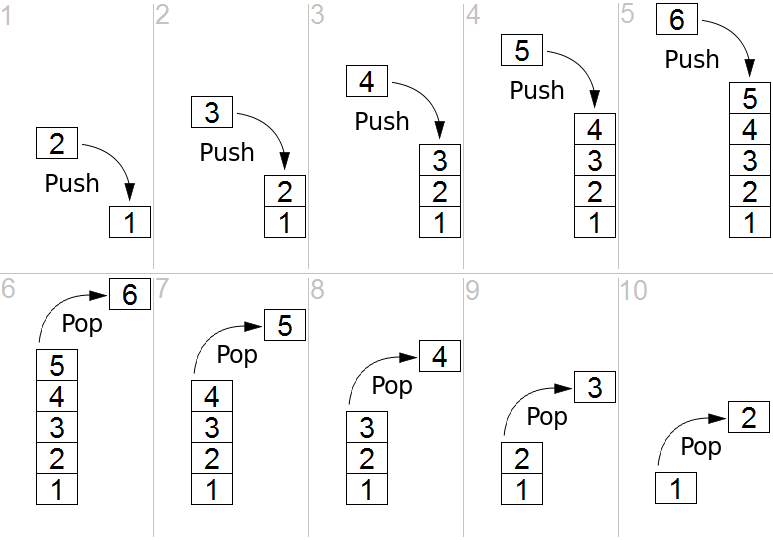
\includegraphics[scale=0.38]{imgs/2-LDS/stack/stack.png}
	\end{figure}	
\end{frame}

\begin{frame}[fragile]{Stack}
    \begin{itemize}
		\item ADT where the main operations are insertion (\textbf{push}) and removal (\textbf{pop}) from the top of the stack
			\begin{itemize}
				\item Top: accessible
				\item Bottom: inaccessible
			\end{itemize}
	\end{itemize}
	
	\begin{figure}
		\centering
		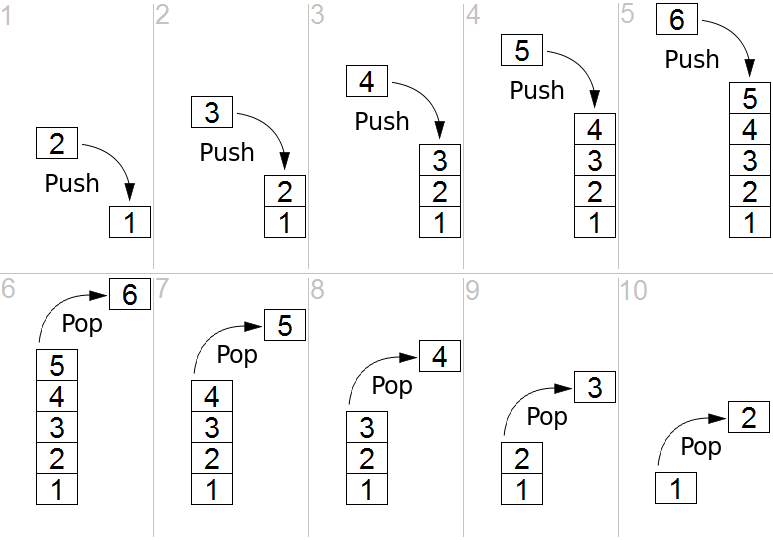
\includegraphics[scale=0.2]{imgs/2-LDS/stack/stack.png}
	\end{figure}	
	
	\begin{itemize}
		\item Last-In-First-Out (LIFO)
		\item Single Linked List where we can only perform insertions and deletions from the top
	\end{itemize}
\end{frame}

\begin{frame}[fragile]
\frametitle{Stack: Applications}
	\begin{itemize}
		\item Bracket Matching:
			$$\{\;[\;(\;(\;(\;)\;)\;)\;]\;\}$$
			$$(\;\{\;[\color{red}\;\{\color{black}\;[\;(\;)\;]\;]\;\}\;)$$
			Are the previous strings valid?
		\item Postfix calculator
			$$2\;3 \;+ \;4 \;*$$
			Is this string a valid sentence ? $\rightarrow (2+3)*4$
	\end{itemize}
\end{frame}


%----------------------------------------------------------------------
%-------------------------------QUEUE----------------------------------
%----------------------------------------------------------------------
\begin{frame}
\frametitle{Queue}
	\begin{figure}
		\centering
		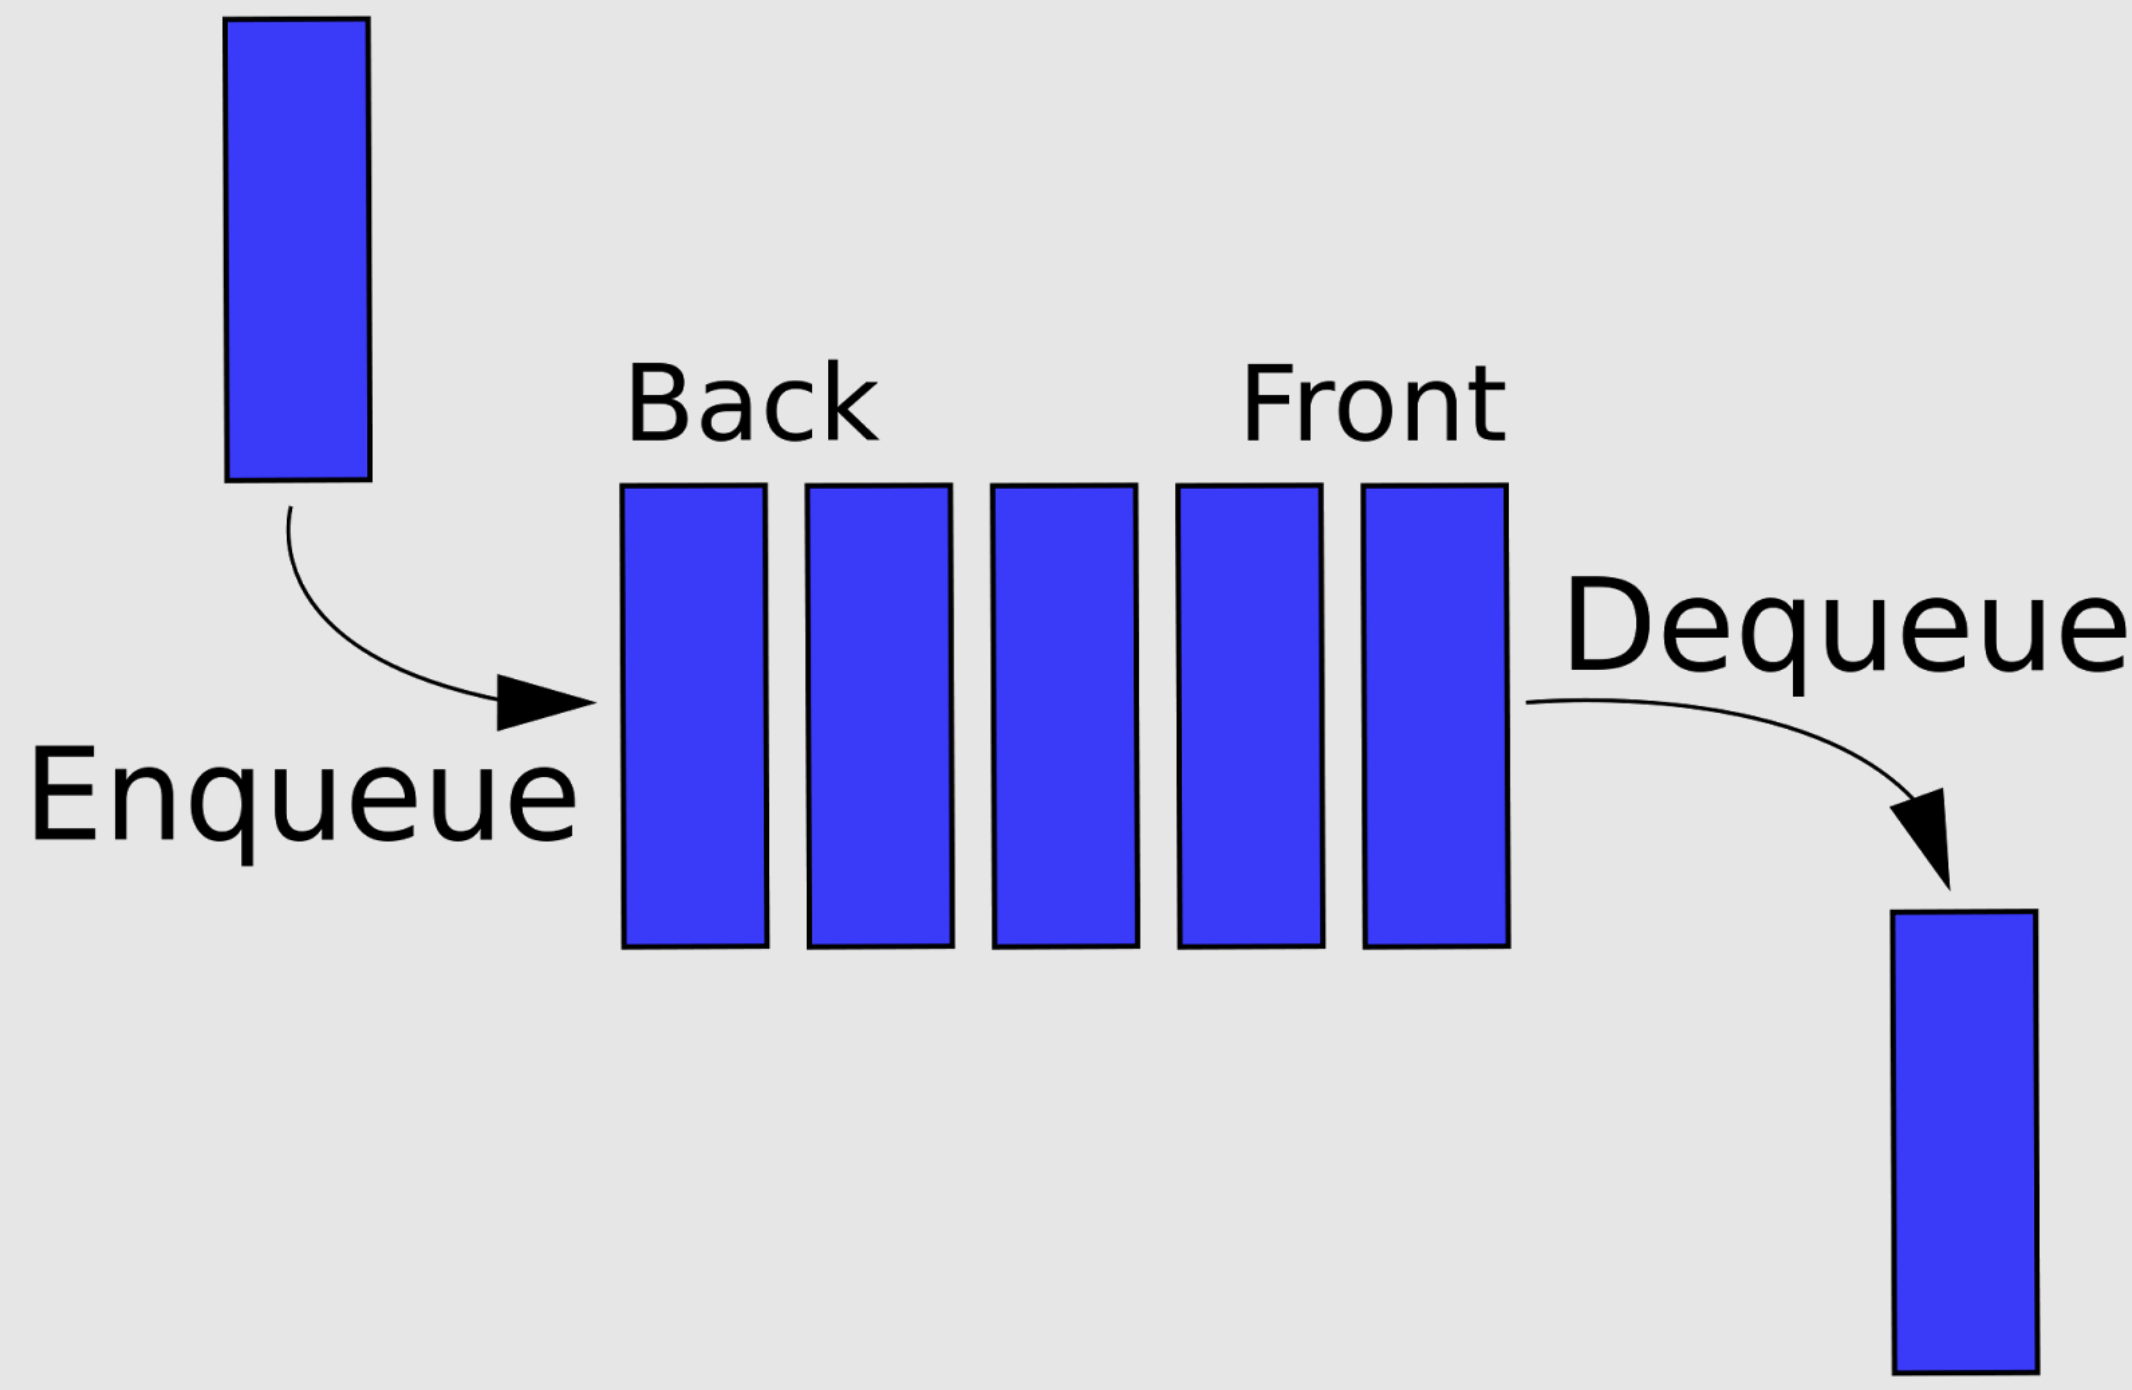
\includegraphics[scale=0.2]{imgs/2-LDS/queue/queue.png}
	\end{figure}
\end{frame}

\begin{frame}[fragile]{Queue}
    \begin{itemize}
    	\item ADT where items in the collection are kept in order and the main operations are addition of items to the back of the queue (\textbf{enqueue}) and removal of items from the front (\textbf{dequeue}) - FIFO
		\begin{figure}
			\centering
			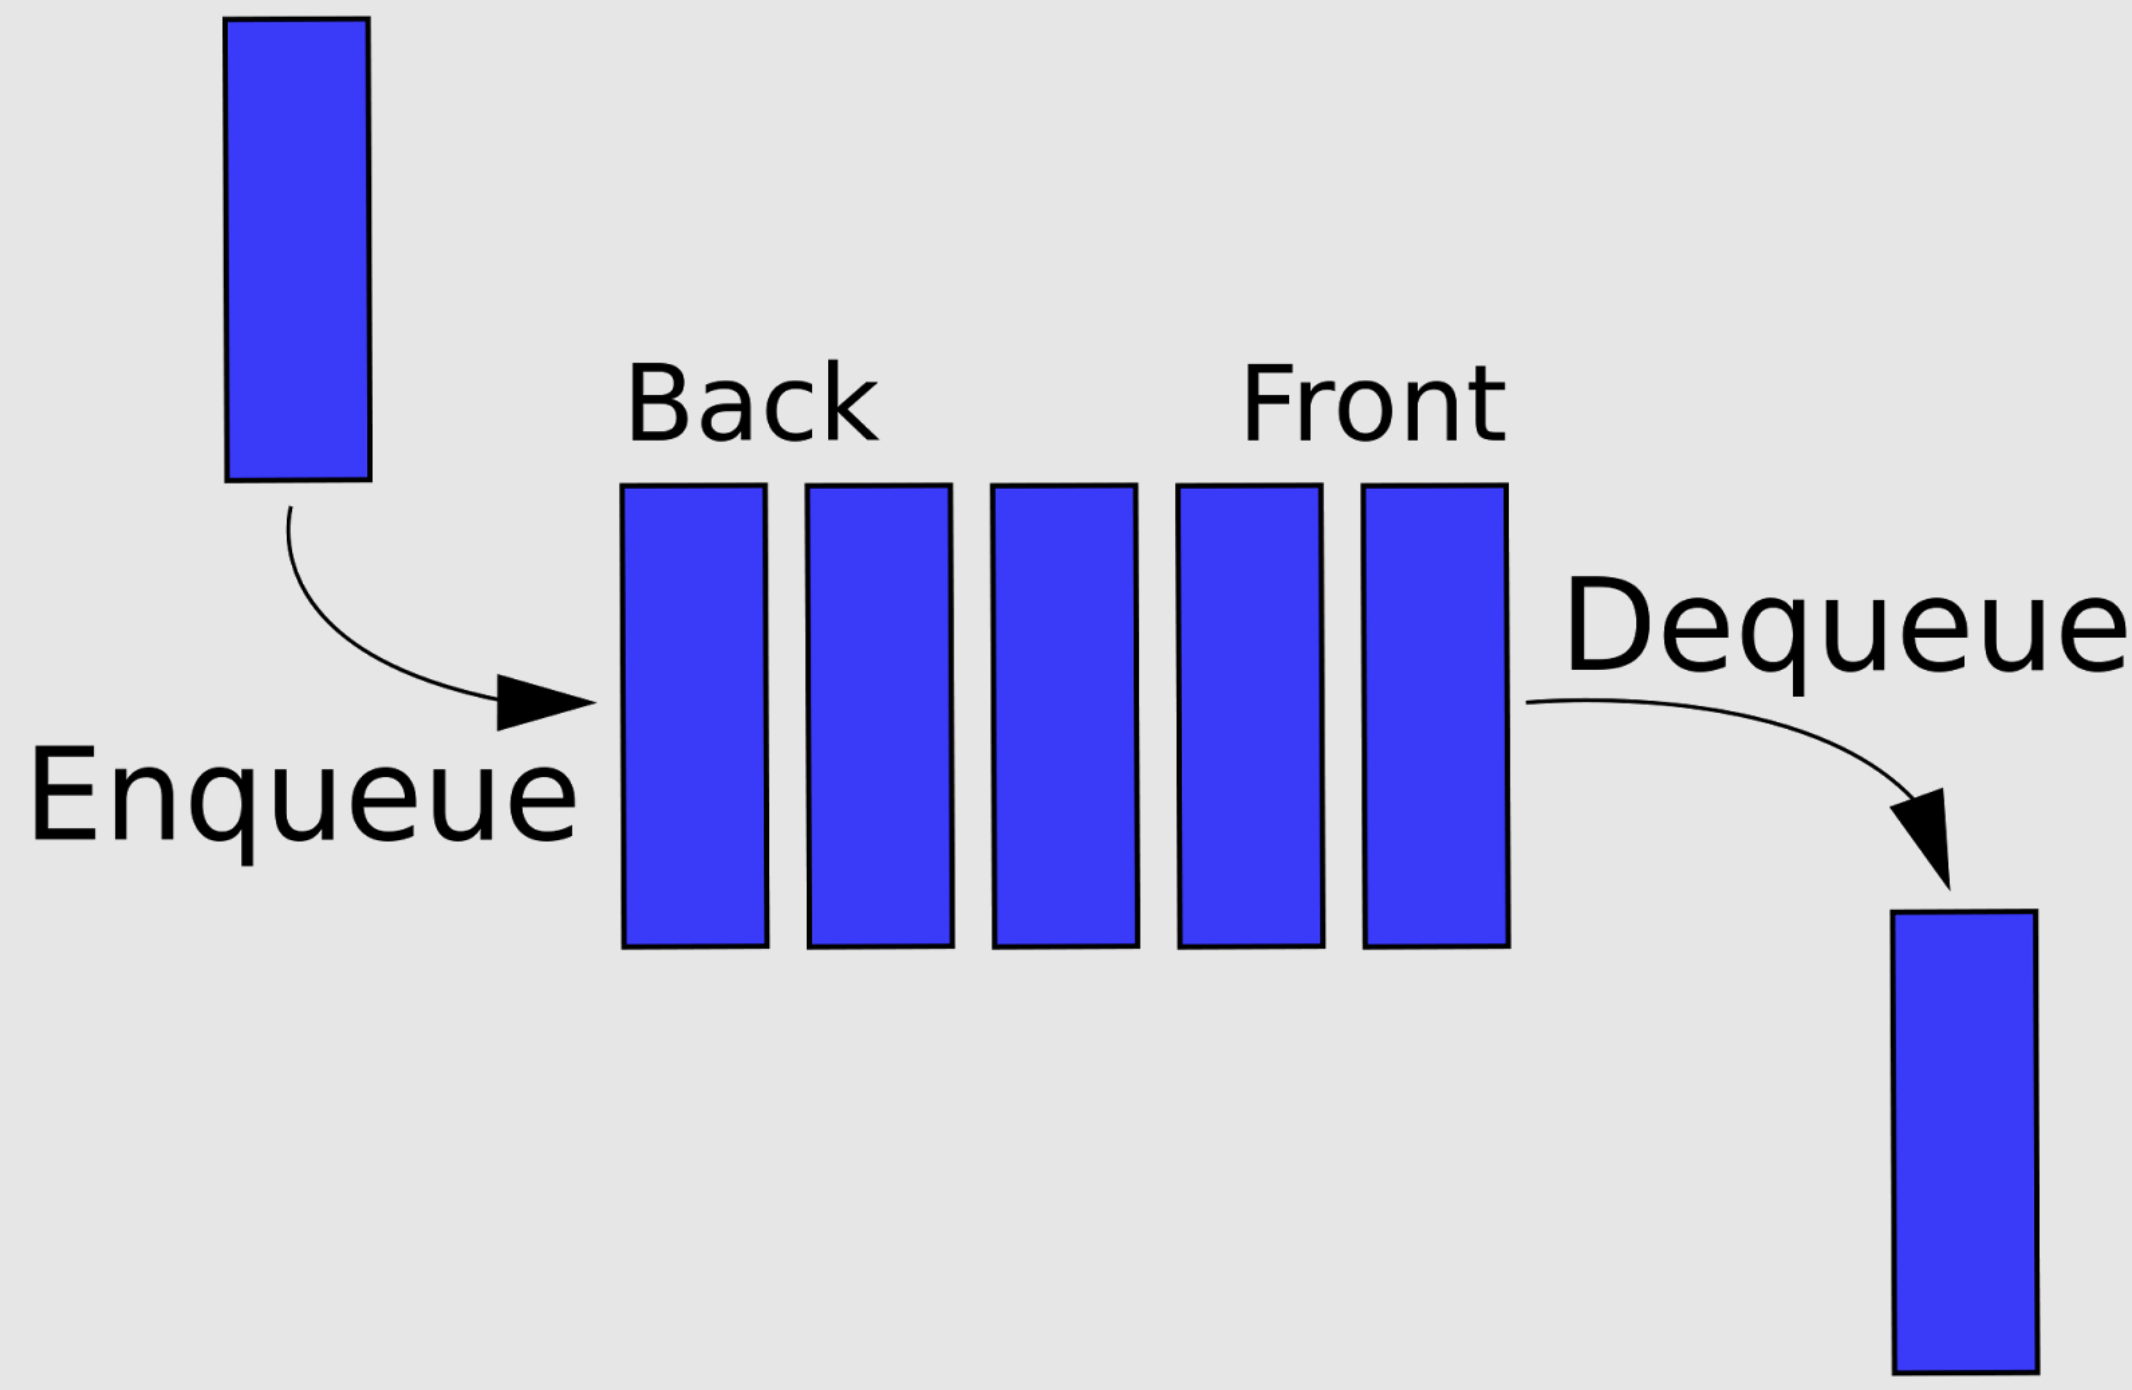
\includegraphics[scale=0.1]{imgs/2-LDS/queue/queue.png}
		\end{figure}
        \item Common implementations of a Queue are with a protected Singly Linked List where both enqueue and dequeue have $O(1)$ complexities
        \item \verb|C++|: \verb|STL queue|
    \end{itemize}
\end{frame}

\begin{frame}
\frametitle{Queue - Applications}
	\begin{itemize}
		\item Simulation of real queues
		\item Breadth-First Search (BFS) algorithm for graph traversal
	\end{itemize}
\end{frame}

%----------------------------------------------------------------------
%-------------------------------DLL------------------------------------
%----------------------------------------------------------------------
\begin{frame}
\frametitle{Doubly Linked List}
	\begin{figure}
		\centering
		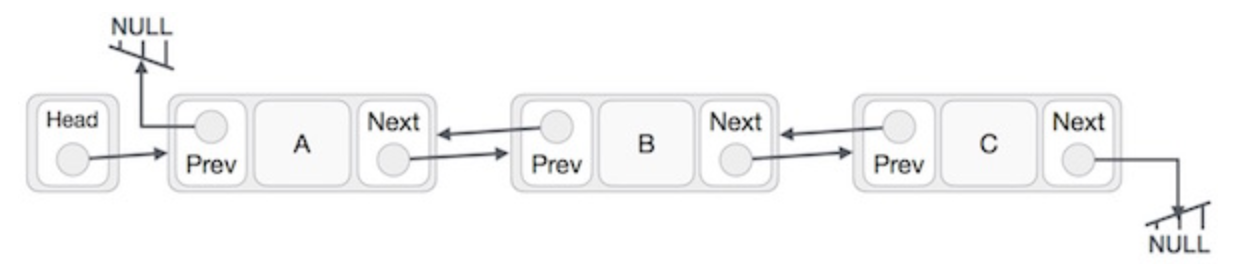
\includegraphics[scale=0.5]{imgs/2-LDS/dll/dll.png}
	\end{figure}
\end{frame}

\begin{frame}[fragile]
\frametitle{Doubly Linked List}
	\begin{itemize}
		\item Each vertex contains two pointers:
			\begin{itemize}
				\item Next
				\item Prev
			\end{itemize}
			\begin{figure}
				\centering
				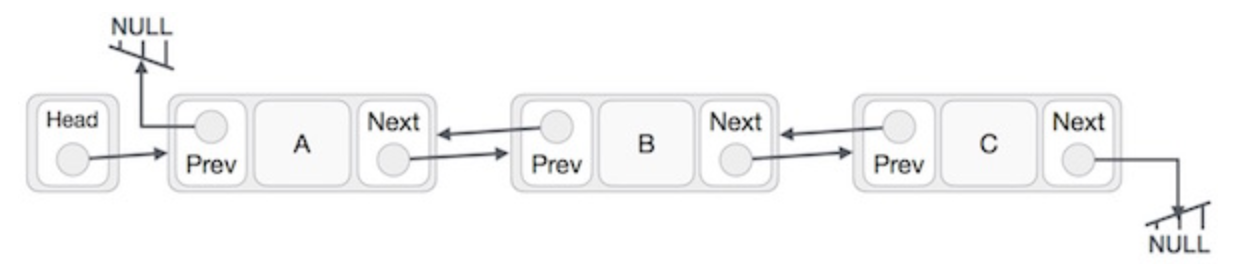
\includegraphics[scale=0.3]{imgs/2-LDS/dll/dll.png}
			\end{figure}
		\item The usage of \textbf{prev} makes it easier to move backwards but DLL occupies two times the memory of a singly LL
		\item \verb|C++ STL: list|
	\end{itemize}
\end{frame}

\begin{frame}[fragile]
\frametitle{Doubly Linked List - Remove at tail}
	\begin{itemize}
		\item One benefit of using \textbf{prev} pointer is the ability to move backwards, which makes the problem of removing the tail element $O(1)$. In a singly LL removing the tail element used linear time since we needed to iterate over the LL until finding the tail
		\item With \textbf{prev} pointer we have direct access to the tail element via the \textbf{tail} pointer and to the previous item via the \textbf{prev} pointer
	\end{itemize}
	\begin{lstlisting}[language=c++]
Vertex *temp = tail;
tail = tail->prev;
tail->next = null;
delete temp;
\end{lstlisting}
\end{frame}


%----------------------------------------------------------------------
%-------------------------------Deque----------------------------------
%----------------------------------------------------------------------
\begin{frame}
\frametitle{Deque}
	\begin{figure}
		\centering
		
\includegraphics[scale=0.4]{imgs/2-LDS/deque/deque.png}
	\end{figure}
\end{frame}

\begin{frame}[fragile]{Deque}
    \begin{itemize}
        \item Doubled Ended Queue. Pronounced "deck"
        \item ADT that generalizes a Queue for which elements can be added to or removed from either the front or the back
		\begin{figure}
			\centering
			
\includegraphics[scale=0.3]{imgs/2-LDS/deque/deque.png}
		\end{figure}
		\item Can be implemented as a protected DLL
        \item \color{red}\verb|C++| code: \verb|ch2_04_stack_queue.cpp|\color{black}
    \end{itemize}
\end{frame}

\begin{frame}[fragile]
\frametitle{Deque - Operations}
	\begin{itemize}
		\item Query the head or tail
		\item Insert a new item to the head or tail
		\item Remove an existing item from the head or tail
		\item All operations are $O(1)$
	\end{itemize}
\end{frame}

\begin{frame}[fragile]
\frametitle{Deque - Applications}
	\begin{itemize}
		\item Finding the shortest paths 0/1-weighted graphs
		\item Sliding window techniques
	\end{itemize}
\end{frame}

%----------------------------------------------------------------------
%----------------------------------BITSET------------------------------
%----------------------------------------------------------------------
\begin{frame}[fragile]{Bitset}
    \begin{itemize}
        \item Array that holds only boolean values
        \item \verb|C++ STL bitset|
    \end{itemize}
\end{frame}

%----------------------------------------------------------------------
%---------------------------------BITMASK------------------------------
%----------------------------------------------------------------------
\begin{frame}
\frametitle{Bitmask}
	\begin{figure}
		\centering
		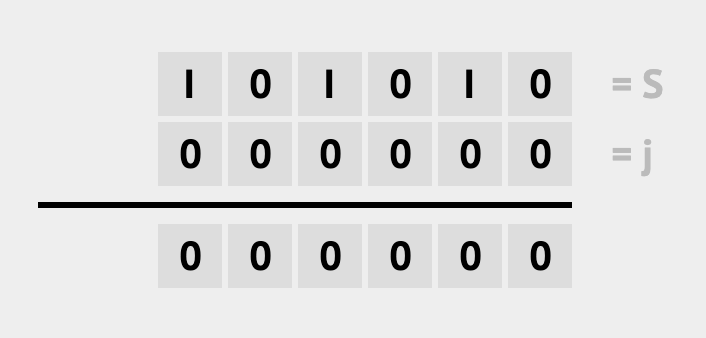
\includegraphics[scale=0.5]{imgs/2-LDS/bitmask/bitmask-operations.png}
		\caption{Input integer \textbf{S}. Bits of the mask \textbf{j}}
	\end{figure}
\end{frame}

\begin{frame}[fragile]{Bitmask}
    \begin{itemize}
        \item Provide an efficient way to manipulate a small set of Booleans
        \item $S$: Input; $j$: bitmask; $O$ is a logical operator applied to $S$ and $j$
        \item Some common operations $O(1)$:
            \begin{itemize}
                \item Multiply and divide by $i$ where $i$ is a power of $2$
                \item Turn on the $j_{th}$ item of the set
                \item Turn off the $j_{th}$ item of the set
                \item Toggle the $j_{th}$ item of the set
                \item Turn on all the bits in a set of size $n$
                \item Check if the $j_{th}$ item is turned on
                \item Get the value of the least significant bit (LSB)
                \item Modulo
                \item Determine if number $m$ is power of $2$
                \item Find nearest power of $2$
                \item Turn off/\color{blue}on \color{black} last bit/\color{blue}zero\color{black}
                \item Turn off/\color{blue}on \color{black} last consecutive bits/\color{blue}zeroes\color{black}
            \end{itemize}
        \item \color{red}\verb|C++| code: \verb|ch2_03_bit_manipulation.cpp|\color{black}            
    \end{itemize}
\end{frame}


%----------------------------------------------------------------------
%---------------------------------Summary------------------------------
%----------------------------------------------------------------------
\begin{frame}{Summary}
	\begin{itemize}
		\item Create operation is the same for LL, Stack, Queue, DLL, Deque
		\item Minor differences for the search/insert/remove operations
			\begin{itemize}
				\item \textbf{Stack}: query/restricted-search, push/restricted-insert and pop/restricted-remove from the top
				\item \textbf{Queue}: query/restricted-search  and pop/restricted-remove from the front. Push/restricted-insert from the back
				\item \textbf{Deque}: query/restricted-search, enqueue/restricted-insert, dequeue/restricted-remove from the front and back but not the middle
				\item \textbf{SLL and DLL}: do not have these restrictions
			\end{itemize}
	\end{itemize}
\end{frame}
	
\begin{frame}{Summary}
    \begin{figure}
        \centering
        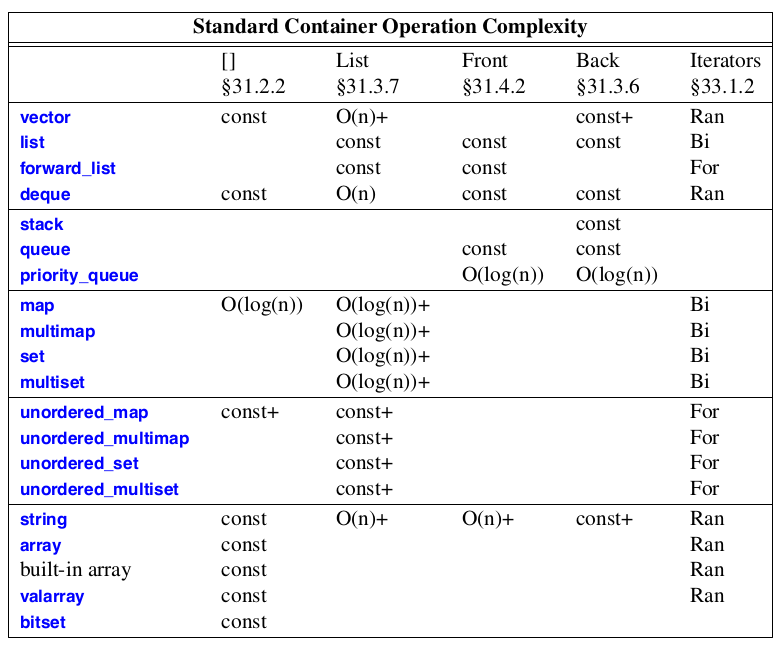
\includegraphics[scale=0.27]{imgs/2-LDS/containers_complexities.png}
        \caption{\textit{Front}: insertion/deletion before the first element. \textit{Back}: insertion/deletion after the last element. \textit{List}: insertions/deletion between front and back}
        \label{fig:lds_summary}
    \end{figure}
\end{frame}

\begin{frame}{Logarithm examples}
    \begin{figure}
        \centering
        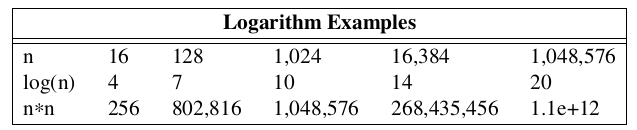
\includegraphics[scale=0.4]{imgs/2-LDS/log_examples.png}
        \caption{"Don’t mess with quadratic algorithms for larger values of $n$"}
        \label{fig:my_label_9}
    \end{figure}
\end{frame}

\begin{frame}{C++ LDS Implementations}
    \begin{figure}
        \centering
        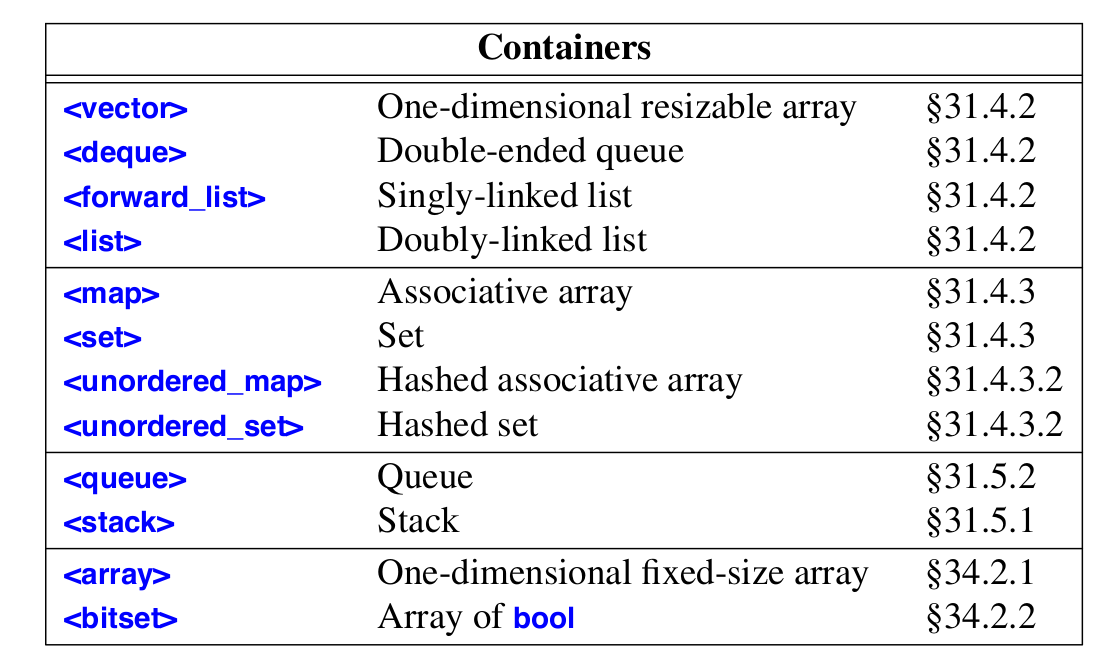
\includegraphics[scale=0.25]{imgs/2-LDS/c++containers.png}
        \caption{Part IV: STL, pg. 863 \cite{Stroustrup}}
        \label{fig:my_label_7}
    \end{figure}
\end{frame}

\begin{frame}{UVa - Competitive Programming 3}
    
    University of Valladolid's Online Judge: 
    
    \url{https://onlinejudge.org/index.php?option=com_onlinejudge&Itemid=8&category=622}
    
    \begin{itemize}
        \item Linear DS with Built In Libraries
    \end{itemize}
\end{frame}

%----------------------------------------------------------------------
%----------------------------------------------------------------------
%----------------------------------------------------------------------
\section{5.2 Ad Hoc Math Problems}

\begin{frame}{Mathematics}
    \begin{itemize}
        \item Most ICPC contests now include problems that need a math insight to be able to find a solution within the given time
        \item The next problems only need basic programming skills and some math fundamentals
    \end{itemize}
\end{frame}

\begin{frame}{Ad Hoc Math Problems}
    \begin{itemize}
        \item Simpler Ones
        \item Simulation (Brute Force)
        \item Finding Pattern or Formula
        \item Grid
        \item Number Systems or Sequences
        \item Logarithm, Exponentiation, Power
        \item Polynomial
        \item Base Number Variants
        \item Ad Hoc
    \end{itemize}
\end{frame}

\begin{frame}{UVa - Competitive Programming 3}
    \url{https://onlinejudge.org/index.php?option=com_onlinejudge&Itemid=8&category=696}
    \begin{itemize}
        \item Ad Hoc Mathematics Problems
    \end{itemize}
\end{frame}


%----------------------------------------------------------------------
%----------------------------------------------------------------------
%----------------------------------------------------------------------
\section{6.2 Basic String Processing Skills}

\begin{frame}{String Processing - Motivation}
    \begin{quote}
        As the strings (e.g. DNA strings) that researchers deal with are usually (very) long, efficient string-specific data structures and algorithms are necessary
    \end{quote}
\end{frame}

\begin{frame}[fragile]{Basic String Processing Skills - \#1}
    \begin{enumerate}
        \item Given a text file that contains only alphabet characters [A-Za-z], digits [0-9], space, and period (‘.’), write a program to read this text file line by line until we encounter a line that starts with seven periods (‘‘.......’’). Concatenate (combine) each line into one long string \verb|T|. When two lines are combined, give one space between them so that the last word of the previous line is separated from the first word of the current line
    \end{enumerate}
\end{frame}

\begin{frame}[fragile]{BSPS - \#2}
    \begin{enumerate}
        \setcounter{enumi}{1}
        \item Suppose that we have one long string \verb|T|. We want to check if another string \verb|P| can be found in \verb|T|. Report all the indices where \verb|P| appears in \verb|T| or report \verb|-1| if \verb|P| cannot be found in \verb|T|
    \end{enumerate}
\end{frame}

\begin{frame}[fragile]{BSPS - \#3}
    \begin{enumerate}
        \setcounter{enumi}{2}
        \item Suppose we want to do some simple analysis of the characters in \verb|T| and also to transform each character in \verb|T| into lowercase. The required analysis are: How many digits, vowels \verb|[aeiouAEIOU]|, and consonants (other alphabets that are not vowels) are there in \verb|T|? Can you do all these in $O(n)$ where $n$ is the length of the string \verb|T|?
    \end{enumerate}
\end{frame}

\begin{frame}[fragile]{BSPS - \#4}
    \begin{enumerate}
        \setcounter{enumi}{3}
        \item Next, we want to break this one long string \verb|T| into tokens (substrings) and store them into an array of strings called \verb|tokens|. For this mini task, the delimiters of these tokens are spaces and periods (thus breaking sentences into words). Then, we want to sort this array of strings lexicographically and then find the lexicographically smallest string
    \end{enumerate}
\end{frame}

\begin{frame}[fragile]{BSPS - \#5}
    \begin{enumerate}
        \setcounter{enumi}{4}
        \item Now, identify which word appears the most in \verb|T|. In order to answer this query, we need to count the frequency of each word. Which data structure should be used for this mini task?
    \end{enumerate}
\end{frame}

\begin{frame}[fragile]{BSPS - \#6}
    \begin{enumerate}
        \setcounter{enumi}{5}
        \item The given text file has one more line after a line that starts with ‘.......’ but the length of this last line is not constrained. Your task is to count how many characters there are in the last line. How to read a string if its length is not known in advance?
    \end{enumerate}
    \begin{itemize}
    \item \color{red}\verb|C++| code: \verb|ch6_01_basic_string.cpp|\color{black}
    \end{itemize}
\end{frame}


%----------------------------------------------------------------------
%----------------------------------------------------------------------
%----------------------------------------------------------------------
\section{6.3 Ad Hoc String Processing Problems}

\begin{frame}{Ad Hoc String Processing Problems}
    \begin{itemize}
        \item Cipher/Encode/Encrypt/Decode/Decrypt
        \item Frequency Counting
        \item Input Parsing
        \item Solvable with Java String/Pattern class (Regular Expression)
        \item Output Formatting
        \item String Comparison
        \item Just Ad Hoc
    \end{itemize}
\end{frame}

\begin{frame}{UVa - Competitive Programming}
    \url{https://onlinejudge.org/index.php?option=com_onlinejudge&Itemid=8&category=737}
    \begin{itemize}
        \item Ad Hoc String Processing Problems
    \end{itemize}
\end{frame}

%----------------------------------------------------------------------
%----------------------------------------------------------------------
%----------------------------------------------------------------------
\section{7.2 Basic Geometry Objects}
\begin{frame}{Overview \& Motivation}
    \begin{itemize}
        \item At least one geometry problem in ICPC
        \item These problems are usually left at the end because are the most time expensive problems and most tedious to code
        \item Main issues with geometry problems:
            \begin{itemize}
                \item Most of them have tricky corner cases
                \item Floating point precision errors
                \item Tedious coding
                \item Contestants forget some basic formulas and are unable to derive more complex formulas
                \item Contestants do not prepare well-written library functions before the contests
            \end{itemize}
    \end{itemize}
\end{frame}

\begin{frame}[fragile]{Basic Geometry Objects with Libraries}
    \begin{itemize}
        \item $0D$ Objects: Points
        \item $1D$ Objects: Lines
        \item $2D$ Objects:
            \begin{itemize}
                \item Circles
                \item Triangles
                \item Quadrilaterals
            \end{itemize}
    \end{itemize}
\end{frame}

\begin{frame}[fragile]{0D - Points}
    \begin{itemize}
        \item Basic building block of higher dimensional geometry objects
        \item Represented with $x$ and $y$ coordinates with respect to the origin $(0,0)$
        \item Features:
            \begin{itemize}
                \item Sort points
                \item Test if two points are equal
                \item Measure the Euclidean distance between two points
                \item Rotate a point by an angle $\theta$ counter clockwise around the origin
            \end{itemize}
    \end{itemize}
\end{frame}

\begin{frame}{1D - Lines}
    \begin{itemize}
        \item Set of points that satisfy the equation: $$Ax + By + C = 0$$
        \item Vertical lines: $B = 1$
        \item Non-vertical lines: $B = 0$
        \item Features: 
            \begin{itemize}
                \item Compute the line equation given at least two points that pass through that line
                \item Test whether two lines are parallel ($A == B$?)
                \item Test whether two lines are the same (both lines must be parallel and their $C$ coefficient must be equal)
                \item Find the intersection point of two lines
            \end{itemize}
    \end{itemize}
\end{frame}

\begin{frame}[fragile]{1D - Lines}
    \begin{itemize}
        \item \textbf{Line Segment}: line with two end points and finite length
        \item \textbf{Vector}: line segment with a direction
        \item More features:
            \begin{itemize}
                \item Translate a point with respect to a vector
                \item Compute the minimum distance from a point $p$ and a line $l$
                \item Compute the minimum distance from a point $p$ and a line segment $ab$. We must consider the end points $a$ and $b$
                \item Compute the angle $aob$ given three points
                \item Determine whether a point $r$ is on the left/right side of a line defined by two points $p$ and $q$ or whether the three points $p, r, q$ are collinear
            \end{itemize}
         \item \color{red} \verb|C++| code: \verb|ch7_01_points_lines.cpp| \color{black}
    \end{itemize}
\end{frame}

\begin{frame}{2D - Circles}
    \begin{itemize}
        \item \textbf{Circle}: centered at coordinate $(a,b)$ with radius $r$ is the set of all points $(x,y)$ such that $(x-a)^2 + (y-b)^2 = r^2$
        \item Safest definition of $\pi$ for a programming contest: $\text{pi} = \text{acos}(-1.0)$ or $\text{pi} = 2*\text{acos}(0.0)$
        \item A circle with radius $r$:
            \begin{itemize}
                \item Diameter $d = 2r$
                \item Circumference $c = 2\pi r$
                \item Area $A = \pi r^2$
            \end{itemize}
        \item \textbf{Arc of a circle}: connected section of the circumference $c$ of the circle.
            \begin{itemize}
                \item Given a central angle $\alpha$ in degrees we can compute the length of the arc as: $$\frac{\alpha}{360.0}\times c$$ 
            \end{itemize}
    \end{itemize}
\end{frame}

\begin{frame}{2D - Circle}
    \begin{itemize}
        \item \textbf{Chord of a circle}: line segment whose endpoints lie on the circle. Line of the chord: $$\sqrt{2r^2\times (1- \cos(\alpha))}$$ Another way: $$2r\sin(\alpha/2)$$
        \item \textbf{Sector of a circle}: region of the circle enclosed by two radius and an arc lying between the two radius. Sector area: $$\frac{\alpha}{360.0}\times A$$
        \item \textbf{Segment} of a circle: region of the circle enclosed by a chord and an arc lying between the chord's endpoints
    \end{itemize}
\end{frame}

\begin{frame}[fragile]{2D - Circle: Features}
    \begin{itemize}
        \item Check if a point is inside, outside or at the border of a circle
        \item Given two points $p_1$ and $p_2$ and radis $r$ determine the location of the centers $c_1$ and $c_2$ of the two possible circles
        \item \color{red} \verb|C++| code: \verb|ch7_02_circles.cpp| \color{black}
    \end{itemize}
\end{frame}

\begin{frame}{2D - Triangles}
    \begin{itemize}
        \item \textbf{Triangle}: polygon with three vertices and three edges
            \begin{itemize}
                \item \textbf{Equilateral}: three equal-length edges and all interior angles of $60$ degrees
                \item \textbf{Isosceles}: two edges have the same length and two interior angles are equal
                \item \textbf{Scalene}: all edges have different lengths
                \item \textbf{Right}: one of its interior angles has $90$ degrees
            \end{itemize}
        \item \textbf{Area}: $A = \frac{b\times h}{2}$
        \item \textbf{Perimeter}: $p = a + b + c$
        \item \textbf{Semiperimeter}: $s = \frac{p}{2}$
        \item \textbf{Heron's Formula}: $A = \sqrt{s\times (s-a)\times (s-b) \times (s-c)}$
        \item \textbf{Inscribed circle} of a triangle has radius $r=\frac{A}{s}$
    \end{itemize}
\end{frame}

\begin{frame}{2D - Triangles}
    \begin{itemize}
        \item \textbf{Circumbrscribed circle}: radius $R = a\times b\times c / (4\times A)$
        \item Check if three line segments $a,b,c$ can form a triangle: $$(a+b>c) \;\&\& (a+c>b) \;\&\& (b+c > a)$$
        \item If the three lengths are sorted, ($a$ smallest and $c$ the largest) we can simply check $$(a+b > c)$$
        \item \textbf{Law of Cosines}: relates the lengths of its sides to the cosine of one of its angles $$\gamma = a\cos (\frac{a^2+b^2 - c^2}{2ab})$$ $$c^2 = a^2 + b^2 -2ab\cos(\gamma)$$
    \end{itemize}
\end{frame}

\begin{frame}{2D - Triangles}
    \begin{itemize}
        \item \textbf{Law of Sines}: relates the lengths of the sides of an arbitrary triangle to the sines of its angle. $$\frac{a}{\sin(\alpha)} = \frac{b}{\sin(\beta)} = \frac{c}{\sin(\gamma} = 2R$$ where $R$ is the radius of the circumcircle
        \item \textbf{Pythagorean Theorem}: only applicable to the right triangles and is a specialization of the Law of Cosines where $\gamma = 90^\circ$ and $\cos(\gamma) = 0$, thus $c^2 = a^2 + b^2$
        \item \textbf{Pythagoream Triple}: triple with three positive integers ($a,b,c$) such that $a^2 + b^2 = c^2$. This triple describes the integer lengths of the three sides of a right triangle. 
    \end{itemize}
\end{frame}

\begin{frame}[fragile]{2D - Triangles - Features}
    \begin{itemize}
        \item Find the center of the incircle: meeting point between the triangle's angel bicectors
        \item Find the center of the circumcircle: meeting point between the triangle's perepdnicular bisectors
		\item \color{red} \verb|C++| code: \verb|ch7_03_triangles.cpp| \color{black}
    \end{itemize}
\end{frame}

\begin{frame}{2D - Quadrilaterals}
    \begin{itemize}
        \item \textbf{Quadrilateral}: polygon with four edges and four vertices
        \item \textbf{Rectangle}: polygon with four edges, four vertices and four right angles
            \begin{itemize}
                \item Area: $A = w\times h$
                \item Perimeter: $P = 2\times (w + h)$
            \end{itemize}
        \item \textbf{Square}: rectangle where $w=h$
        \item \textbf{Trapezium}: polygon with four edges, four vertices and one pair of parallel edges
            \begin{itemize}
                \item Area: $A = \frac{1}{2} \times (w_1 + w_2) \times h$ where $w_i$ is the length of the edge $i$ from the parallel edges and $h$ is the height between those parallel edges
                \item \textbf{Isosceles Trapezium}: the two non-parallel sides have the same length
            \end{itemize}
    \end{itemize}
\end{frame}

\begin{frame}{2D - Queadrilaterals}
    \begin{itemize}
        \item \textbf{Parallelogram}: polygon with four edges and four vertices and the opposite sides must be parallel
        \item \textbf{Kite}: quadrilateral with two pairs of sides of the same length which are adjacent to each other. Area: $A = (D_1 \times D_2 )/2$
        \item \textbf{Rhombus}: special parallelogram where each side has the same length and a special case of a kite where each side has the same length
    \end{itemize}
\end{frame}

\begin{frame}{UVa - Competitive Programming 3}
    \url{https://onlinejudge.org/index.php?option=com_onlinejudge&Itemid=8&category=756}
    \begin{itemize}
        \item Basic Geometry
    \end{itemize}
\end{frame}

%----------------------------------------------------------------------
%----------------------------------------------------------------------
%----------------------------------------------------------------------
\section*{References}
\begin{frame}{References}
    \begin{thebibliography}{}
        \bibitem[Halim]{Halim} Halim S., Halim F., \textit{Competitive Programming 3}, Handbook for ACM ICPC and IOI Contestants. 2013
        \bibitem[Stroustrup]{Stroustrup} Stroustrup B. \textit{The C++ Programming Language}. Fourth ed. 
        \bibitem{skiena} Skiena S. \textit{The Algorithm Design Manual}. Springer. 2020
    \end{thebibliography}
\end{frame}

\end{document}